%!TEX root = ../thesis.tex
% ******************************* Thesis Appendix E ********************************

\chapter{GEANT4 Light Output Vs. Fitted Light Output}

\begin{figure}[htbp]
\centering
\begin{subfigure}{.49\textwidth}
  \centering
  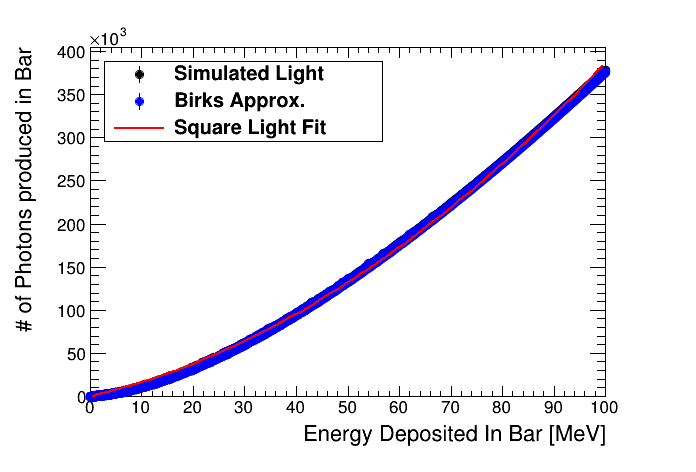
\includegraphics[width=\linewidth]{Appendix5/newFigs/alphaBirksSlab_simAndApproxLight.png}
  \captionsetup{width=.9\linewidth}
  \caption{Simulated 1E6 $\alpha$ particles.}
  \label{subfig:append5_light_of_Alphas0-100mev}
\end{subfigure}
\begin{subfigure}{.49\textwidth}
  \centering
  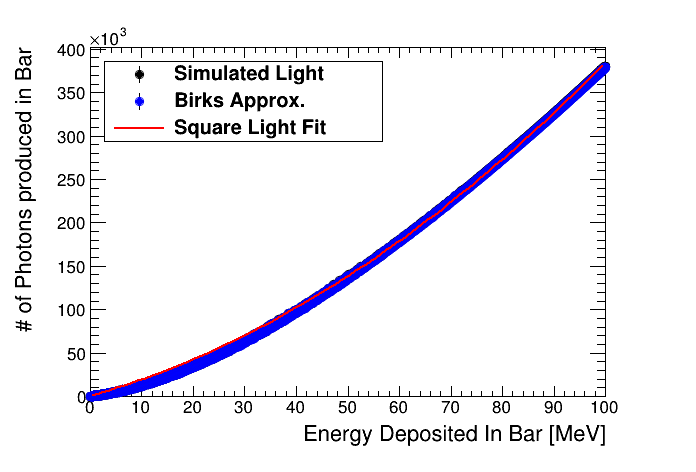
\includegraphics[width=\linewidth]{Appendix5/newFigs/aAlphaBirksSlab_simAndApproxLight.png}
  \captionsetup{width=.9\linewidth}
  \caption{Simulated 1E6 $\bar{\alpha}$ particles.}
  \label{subfig:append5_light_of_AAlphas0-100mev}
\end{subfigure}
\caption{How the Birks approximation (equation \ref{equ:Birks_formula}) approximates light for alpha particles. The Birks approximation is very suitable for these particles.}
\label{fig:append5_light_of_Alphas_AAlphas0-100mev}
\end{figure}

\begin{figure}[htbp]
\centering
\begin{subfigure}{.5\textwidth}
  \centering
  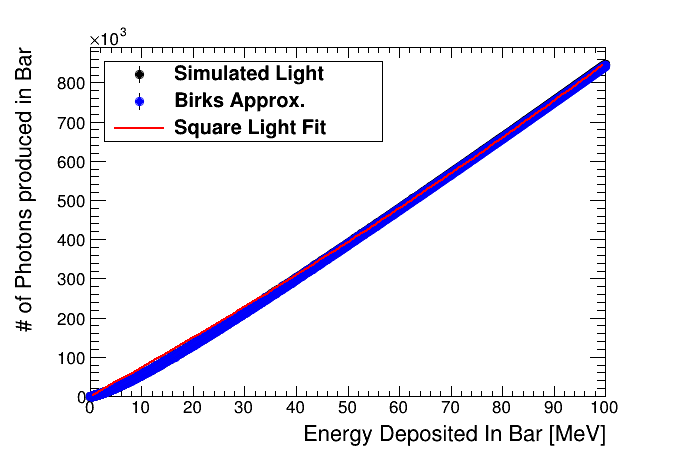
\includegraphics[width=\linewidth]{Appendix5/newFigs/protonBirksSlab_simAndApproxLight.png}
  \captionsetup{width=.9\linewidth}
  \caption{Simulated 1E6 proton particles.}
  \label{subfig:append5_light_of_protons0-100mev}
\end{subfigure}%
\begin{subfigure}{.5\textwidth}
  \centering
  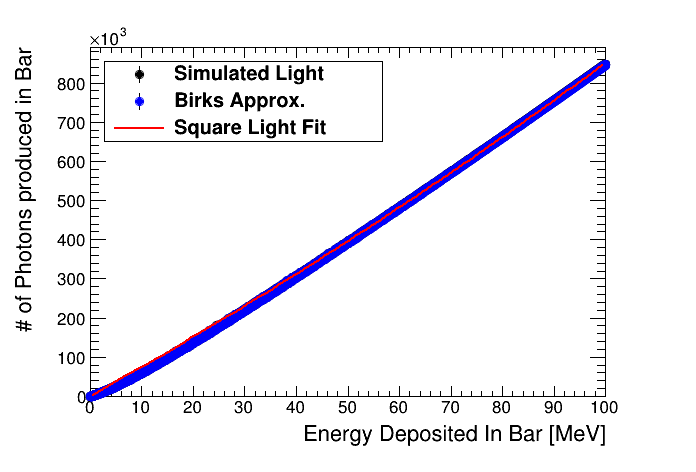
\includegraphics[width=\linewidth]{Appendix5/newFigs/aProtonBirksSlab_simAndApproxLight.png}
  \captionsetup{width=.9\linewidth}
  \caption{Simulated 1E6 anti-proton particles.}
  \label{subfig:append5_light_of_Aprotons0-100mev}
\end{subfigure}
\caption{How the Birks approximation (equation \ref{equ:Birks_formula}) approximates light for protons and anti-protons. The Birks approximation is very suitable for these particles.}
\label{fig:append5_light_of_protons_Aprotons0-100mev}
\end{figure}

\begin{figure}[htbp]
\centering
\begin{subfigure}{.5\textwidth}
  \centering
  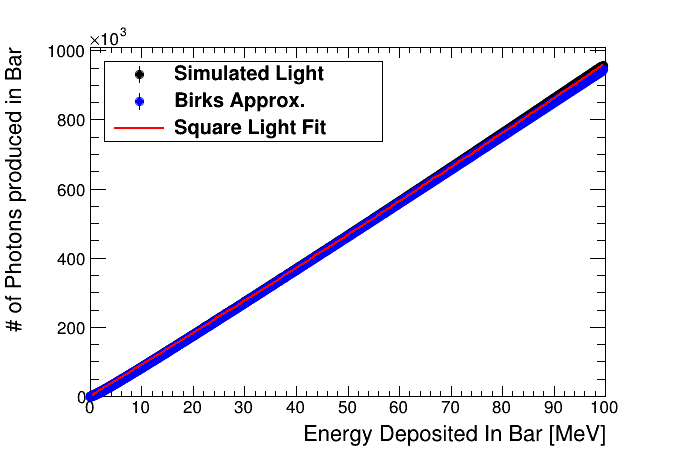
\includegraphics[width=\linewidth]{Appendix5/newFigs/pi+BirksSlab_simAndApproxLight.png}
  \captionsetup{width=.9\linewidth}
  \caption{Simulated 1E6 $\pi^+$ particles.}
  \label{subfig:append5_light_of_pIPlus0-100mev}
\end{subfigure}%
\begin{subfigure}{.5\textwidth}
  \centering
  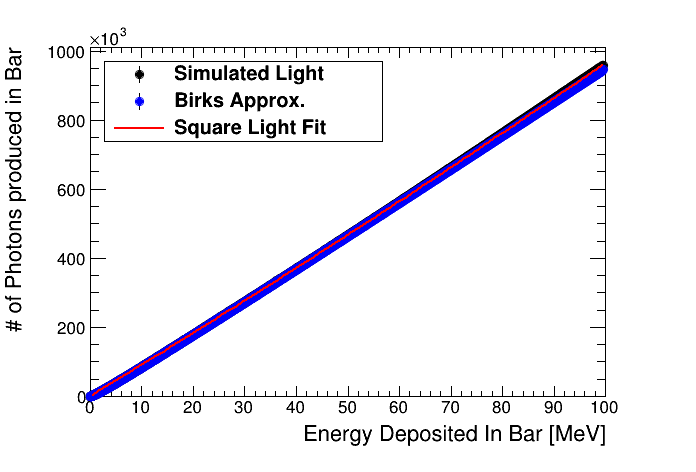
\includegraphics[width=\linewidth]{Appendix5/newFigs/pi-BirksSlab_simAndApproxLight.png}
  \captionsetup{width=.9\linewidth}
  \caption{Simulated 1E6 $\pi^-$ particles.}
  \label{subfig:append5_light_of_pIMinus0-100mev}
\end{subfigure}
\caption{How the Birks approximation (equation \ref{equ:Birks_formula}) approximates light for $\pi^+$ and $\pi^-$.}
\label{fig:append5_light_of_pIPlus_pIMinus0-100mev}
\end{figure}

\begin{figure}[htbp]
\centering
\begin{subfigure}{.5\textwidth}
  \centering
  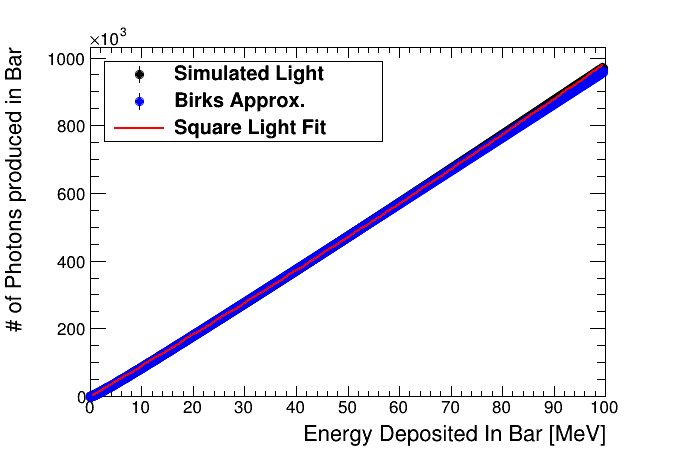
\includegraphics[width=\linewidth]{Appendix5/newFigs/mu-BirksSlab_simAndApproxLight.png}
  \captionsetup{width=.9\linewidth}
  \caption{Simulated 1E6 $\mu^-$ particles.}
  \label{subfig:append5_light_of_muons0-100mev}
\end{subfigure}%
\begin{subfigure}{.5\textwidth}
  \centering
  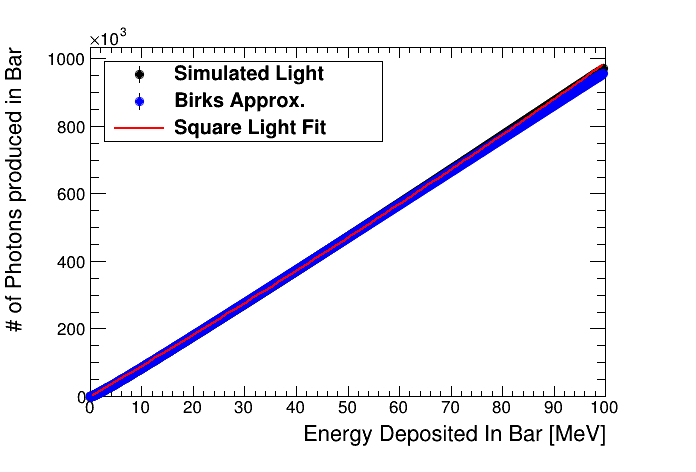
\includegraphics[width=\linewidth]{Appendix5/newFigs/mu+BirksSlab_simAndApproxLight.png}
  \captionsetup{width=.9\linewidth}
  \caption{Simulated 1E6 $\mu^+$ particles.}
  \label{subfig:append5_light_of_Amuons0-100mev}
\end{subfigure}
\caption{How the Birks approximation (equation \ref{equ:Birks_formula}) approximates light for $\mu^-$ and $\mu^+$. The Birks approximation is very suitable for these particles.}
\label{fig:append5_light_of_muons_Amuons0-100mev}
\end{figure}

\begin{figure}[htbp]
\centering
\begin{subfigure}{.5\textwidth}
  \centering
  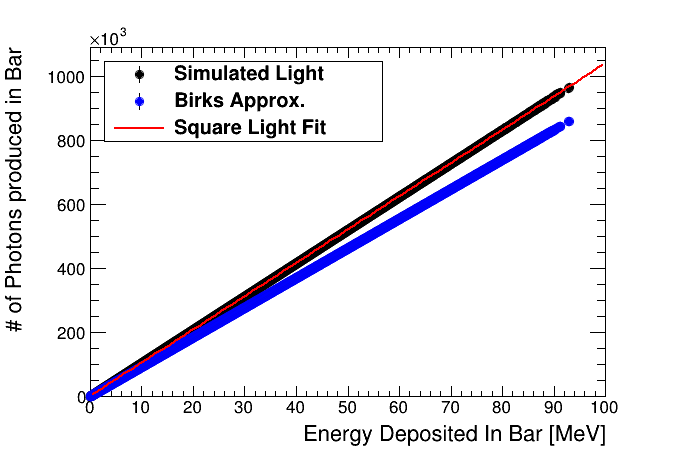
\includegraphics[width=\linewidth]{Appendix5/newFigs/e-BirksSlab_simAndApproxLight.png}
  \captionsetup{width=.9\linewidth}
  \caption{Simulated 1E6 $e^-$ particles.}
  \label{subfig:append5_light_of_electrons0-100mev}
\end{subfigure}%
\begin{subfigure}{.5\textwidth}
  \centering
  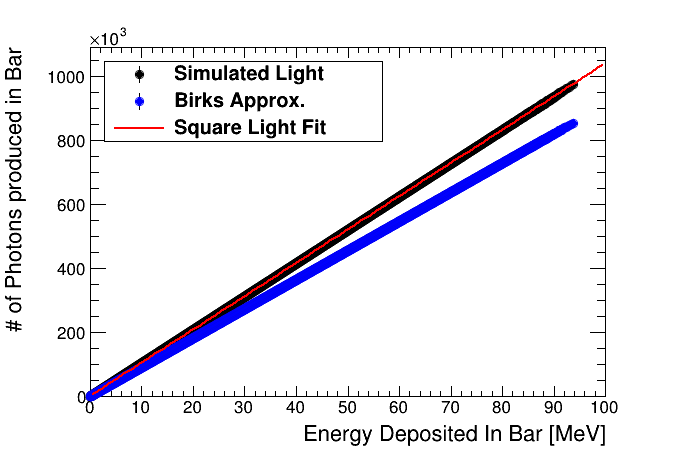
\includegraphics[width=\linewidth]{Appendix5/newFigs/e+BirksSlab_simAndApproxLight.png}
  \captionsetup{width=.9\linewidth}
  \caption{Simulated 1E6 $e^+$ particles.}
  \label{subfig:append5_light_of_positrons0-100mev}
\end{subfigure}
\caption{How the Birks approximation (equation \ref{equ:Birks_formula}) approximates light for e$^-$ and $e^+$. The Birks approximation is unsuitable.}
\label{fig:append5_light_of_electrons_positrons0-100mev}
\end{figure}

\begin{figure}[htbp]
\centering
\begin{subfigure}{.5\textwidth}
  \centering
  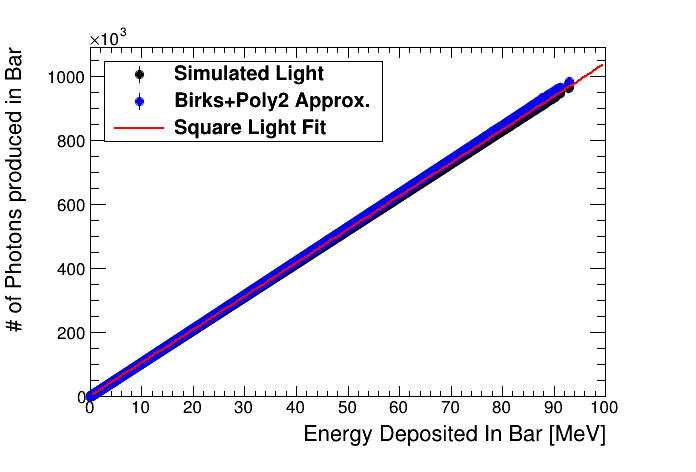
\includegraphics[width=\linewidth]{Appendix5/newFigs/e-Birks-Poly2Slab_simAndApproxLight.png}
  \captionsetup{width=.9\linewidth}
  \caption{}
  \label{subfig:append5_light_of_electronsLin0-100mev}
\end{subfigure}%
\begin{subfigure}{.5\textwidth}
  \centering
  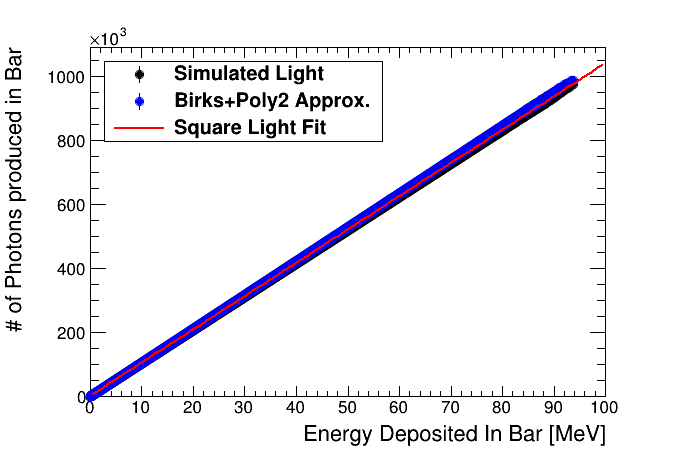
\includegraphics[width=\linewidth]{Appendix5/newFigs/e+Birks-Poly2Slab_simAndApproxLight.png}
  \captionsetup{width=.9\linewidth}
  \caption{}
  \label{subfig:append5_light_of_positronsLin0-100mev}
\end{subfigure}
\caption{The simulated light for 1E6 e$^-$ particles in (a) and 1E6 e$^+$ particles in (b). The approximation for $dE/dx$ is a combination of the Birks law for high values of $dE/dx$ (2 and above) and a polynomial 2 fit between 0-2. Thus approximating the light successfully.}
\label{fig:append5_light_of_electrons_positronsLin0-100mev}
\end{figure}